\section{Visualization Tools}

Visualization tools are supposed to supplement the domain expertise and deliver a big image so that users can frame critical questions and later propose heuristic and insightful answers to these questions \cite{kung2015visualization}. Traditional tools like Excel can not or at least struggle to perform visual analytics on big data involving millions of records so new visualization tools or enhancements in existing tools need to handle the complexity of big data \cite{nair2016interactive}. Dozens, if not hundreds of tools are available to create a visualization of large data sets. Most of them are basic and have a lot of overlapping tools. One way to categorize tools is whether they are drag and drop types or they require coding for creating a visualization. Most of the proprietary visualization tools are of the drag and drop type, which requires no coding skills. Although it is easy to learn and create visualizations in minutes the drawback is that out-of-box visualizations are not possible \cite{nair2016interactive}. In this section, the focus is on the standouts that either have more capability for the types of visualizations they can create and the amount of freedom in customization they can offer or are significantly easier to use than the other options out there. 

\subsection{Tableau}

Tableau is a leading data visualization tool used for data analysis and business intelligence. It is capable of delivering interactive visualizations in no time with its drag and drop nature. Gartner’s Magic Quadrant classified Tableau as a leader for analytics and business intelligence \cite{parenteau2016magic}. Tableau is a user-friendly tool and was built for a diverse number of teams. It is an easy-to-use tool that requires no programming skills and it provides results in a wide variety of formats. It can be connected to the data stored in excel, CSV, and text files and can recognize fields and formats. Moreover, it provides integration with all the major advanced databases, including Teradata, SAP, MySQL, Amazon AWS, and Hadoop. Below are some of the main advantages and disadvantages of using Tableau to visualize big data. To meet the need of diverse users, Tableau software provides selections that include Tableau Desktop, Tableau Server, and Tableau Mobile to choose from. As Tableau Desktop is preferred by individuals and small organizations, Tableau Server is more convenient for big organizations with many users.

On the other hand, it is a very expensive product to scale across huge organizations. Moreover, it provides very basic prepossessing so in most cases data needs to be exported in perfect tables. Finally, no out-of-the-box visualizations can be provided and users have to stick to the offered options.


\begin{figure}[H]
\centering
\captionsetup{justification=centering}
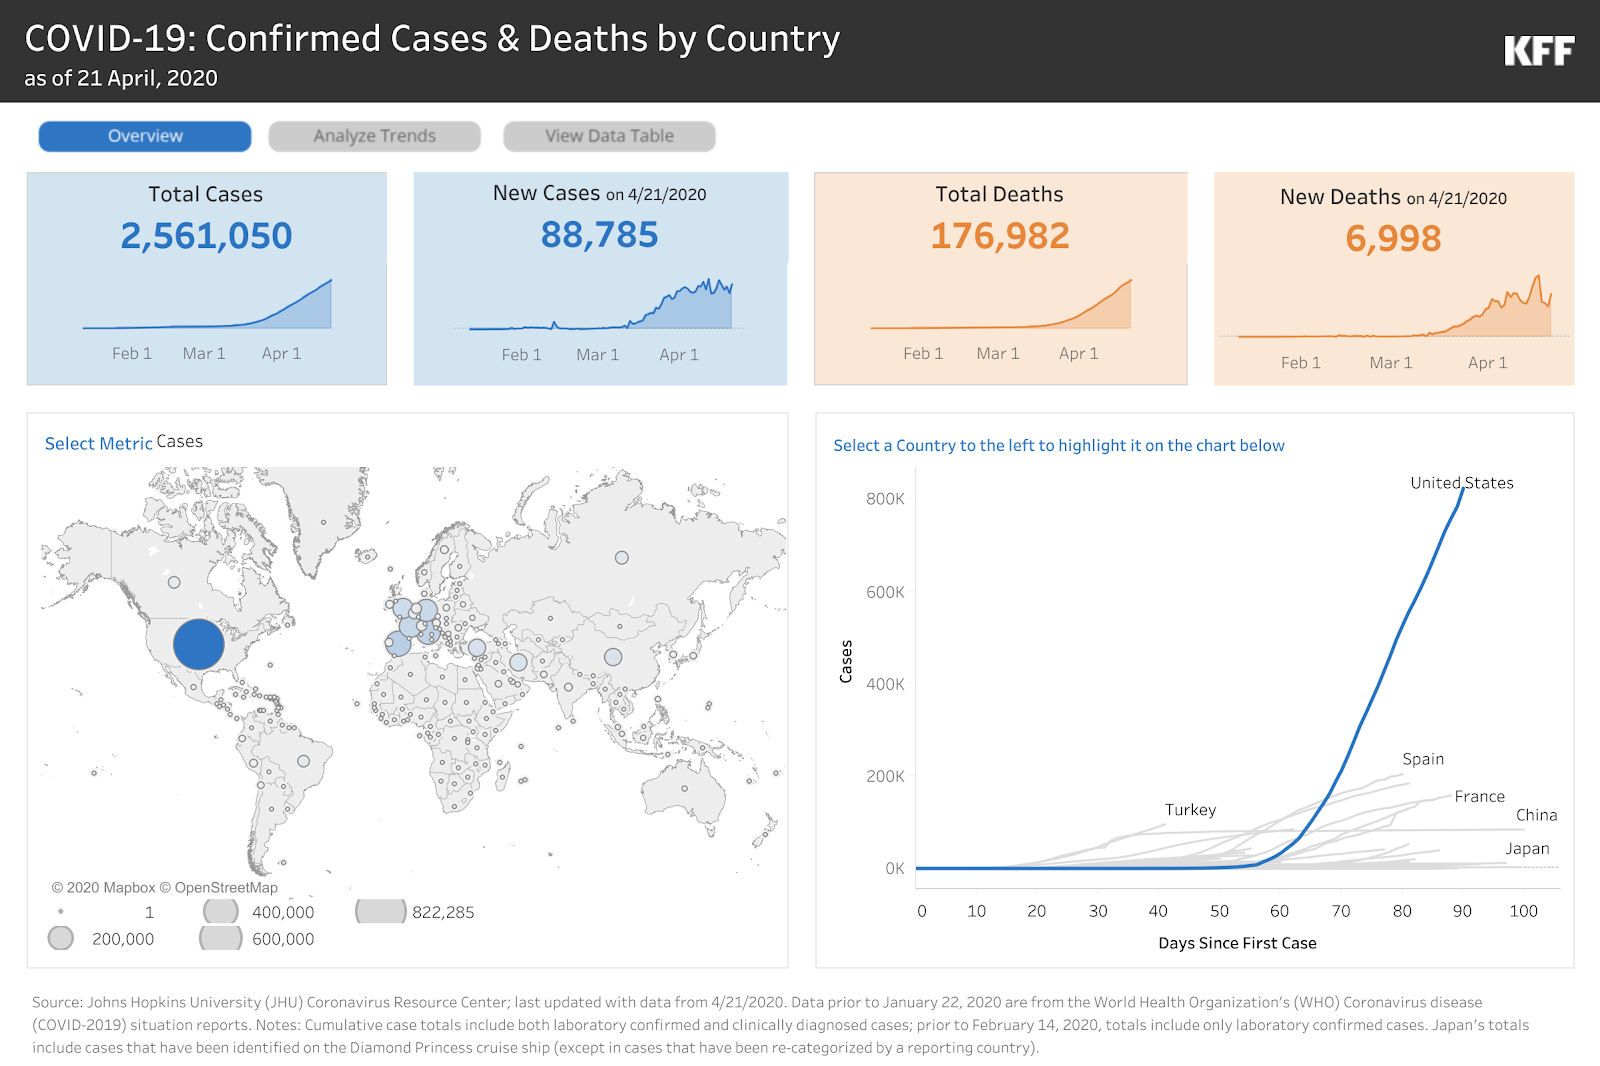
\includegraphics[width=0.9\textwidth]{./pics/tableau.png}
\caption{Tableau dashboard example from (JHU) Coronavirus resource center \cite{kff}}
\label{fig:tableau}
\end{figure}



\subsection{D3.js}

D3 stands for data-driven-documents \cite{2011-d3} and is a free open source tool that makes any visualization possible and in fact, many visualization libraries where JavaScript is the coding language are built on top of D3. D3 outperforms all other JavaScript-based tools as it offers versatile functionalities like data manipulation and transformation and makes effective use of the power of new browser and web technologies \cite{nair2016interactive}. It can create very powerful and highly interactive visualizations. As it requires coding skills in JavaScript, CSS, and HTML any basic visualization needs to be coded from scratch. However, D3 has a big community and many built-in reusable functions, and samples of commonly used graphics are available. D3 can create any imaginable visualization and offers excellent interactivity within coding limits. 

Not supporting older browsers and the programming experience needed to even create simple visualizations are some of the disadvantages that would hold users from using D3. Usually, easier tools with fewer lines of codes would be used unless customization and performance are priorities, especially with big data. 

\begin{figure}[H]
\centering
\captionsetup{justification=centering}
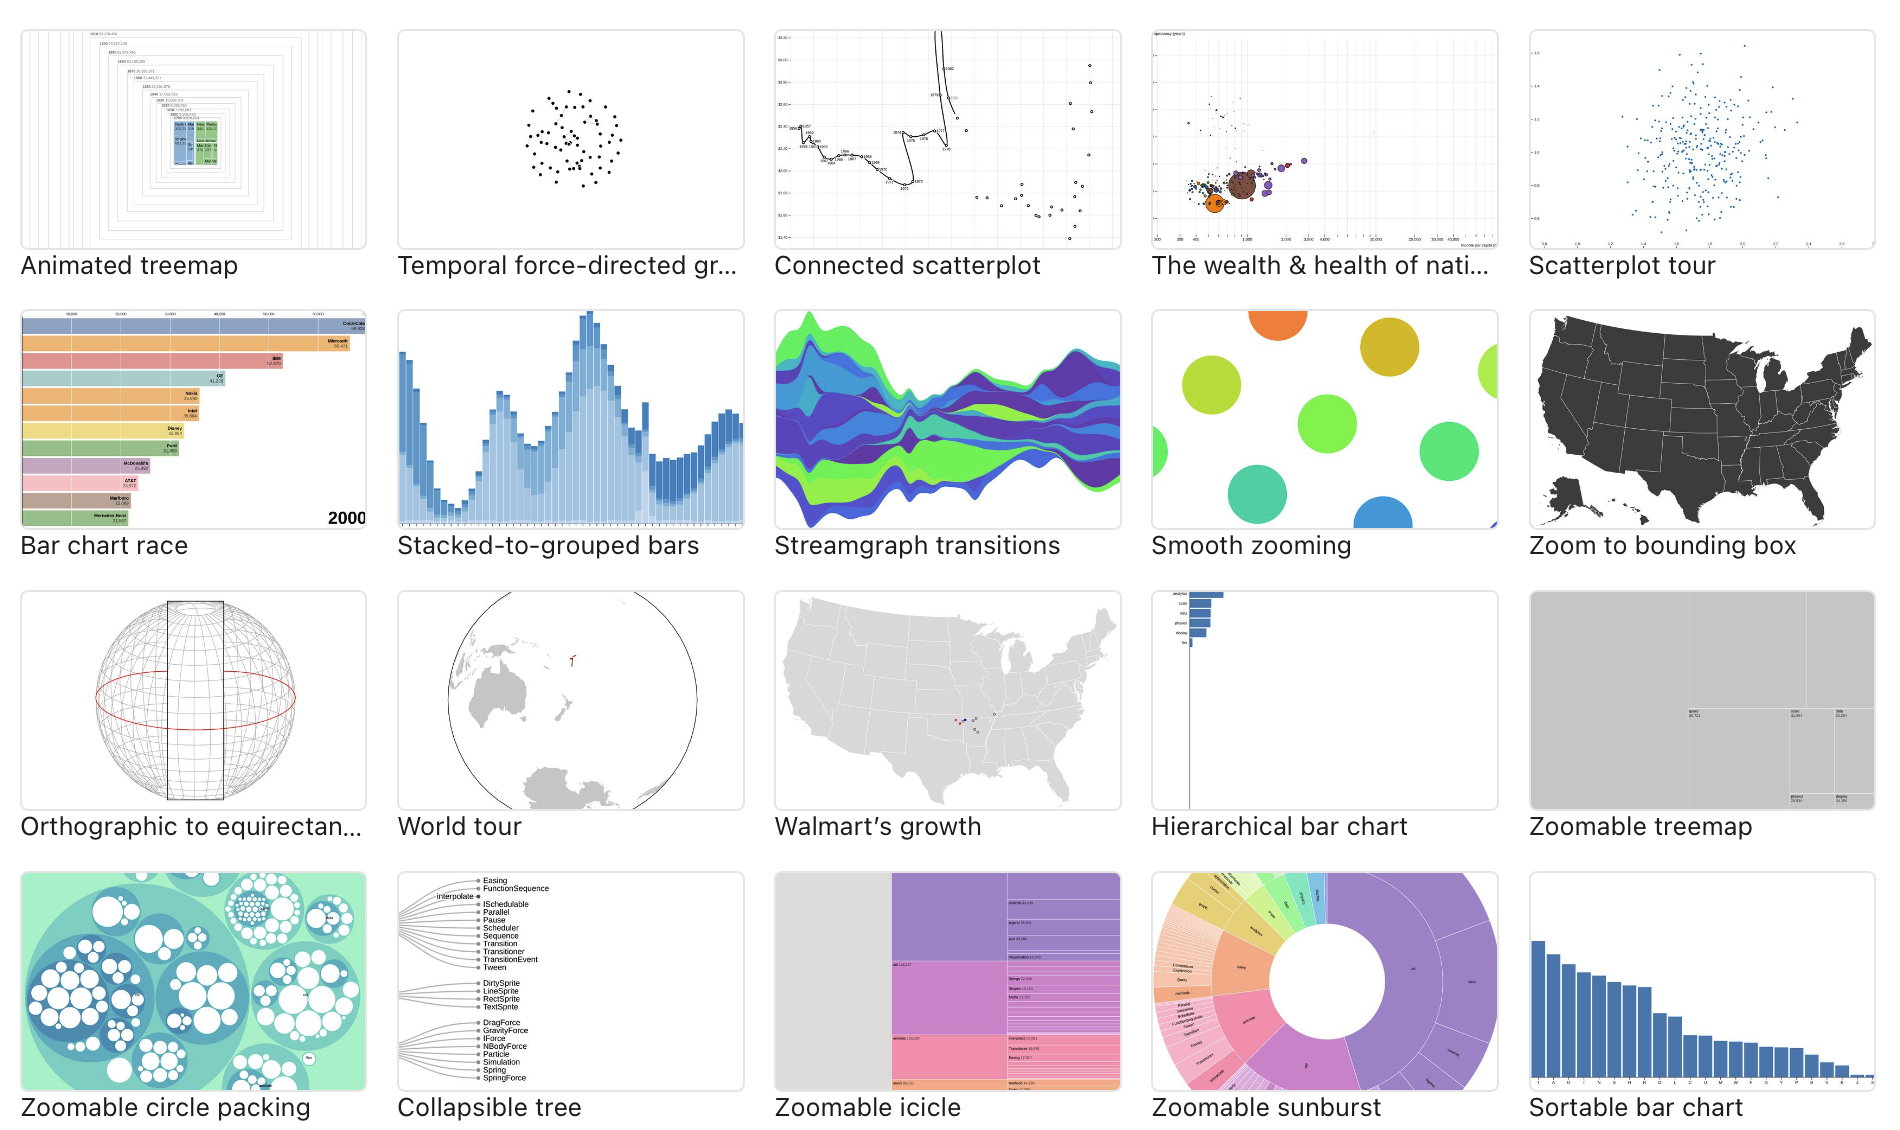
\includegraphics[width=0.9\textwidth]{./pics/d3.png}
\caption{D3 Gallery \cite{d3g}}
\label{fig:d3}
\end{figure}

% \\\  You cannot do this in TeX! RAAZ

\begin{figure}[H]
\centering
\captionsetup{justification=centering}
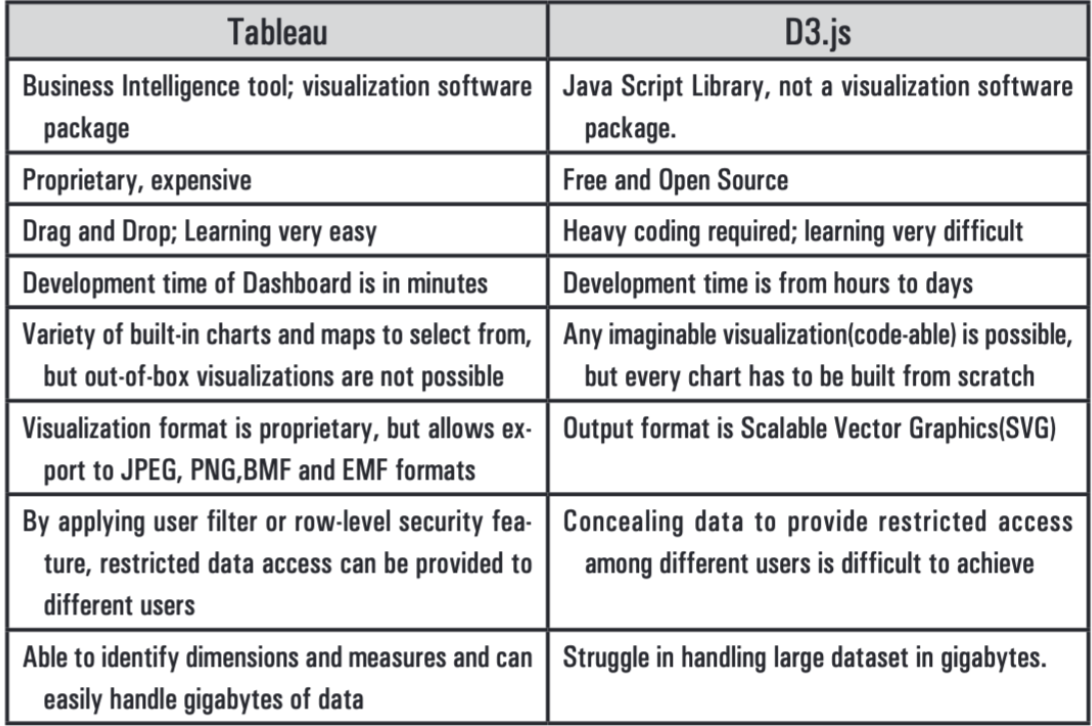
\includegraphics[width=0.7\textwidth]{./pics/tVd3.png}
\caption{Tableau vs D3 \cite{nair2016interactive}}
\label{fig:tableauvsd3}
\end{figure}

\subsection{Vega \& Vega-Lite}

Vega is a visualization tool based on D3 \cite{2016-reactive-vega-architecture}. Vega is a declarative language for creating interactive visualizations. The user can describe the visual appearance and the interaction behavior of the visualization in a JSON format. Vega processes the JSON object and produces the visualization on the browser. On the other hand, Vega-Lite is a high-level visualization tool based on Vega \cite{2017-vega-lite}. Compared to Vega, Vega-Lite is easier and requires fewer lines of codes however it comes with less customization.

\begin{figure}[H]
\begin{subfigure}{.45\textwidth}
  \centering
  \captionsetup{justification=centering}
  % include first image
  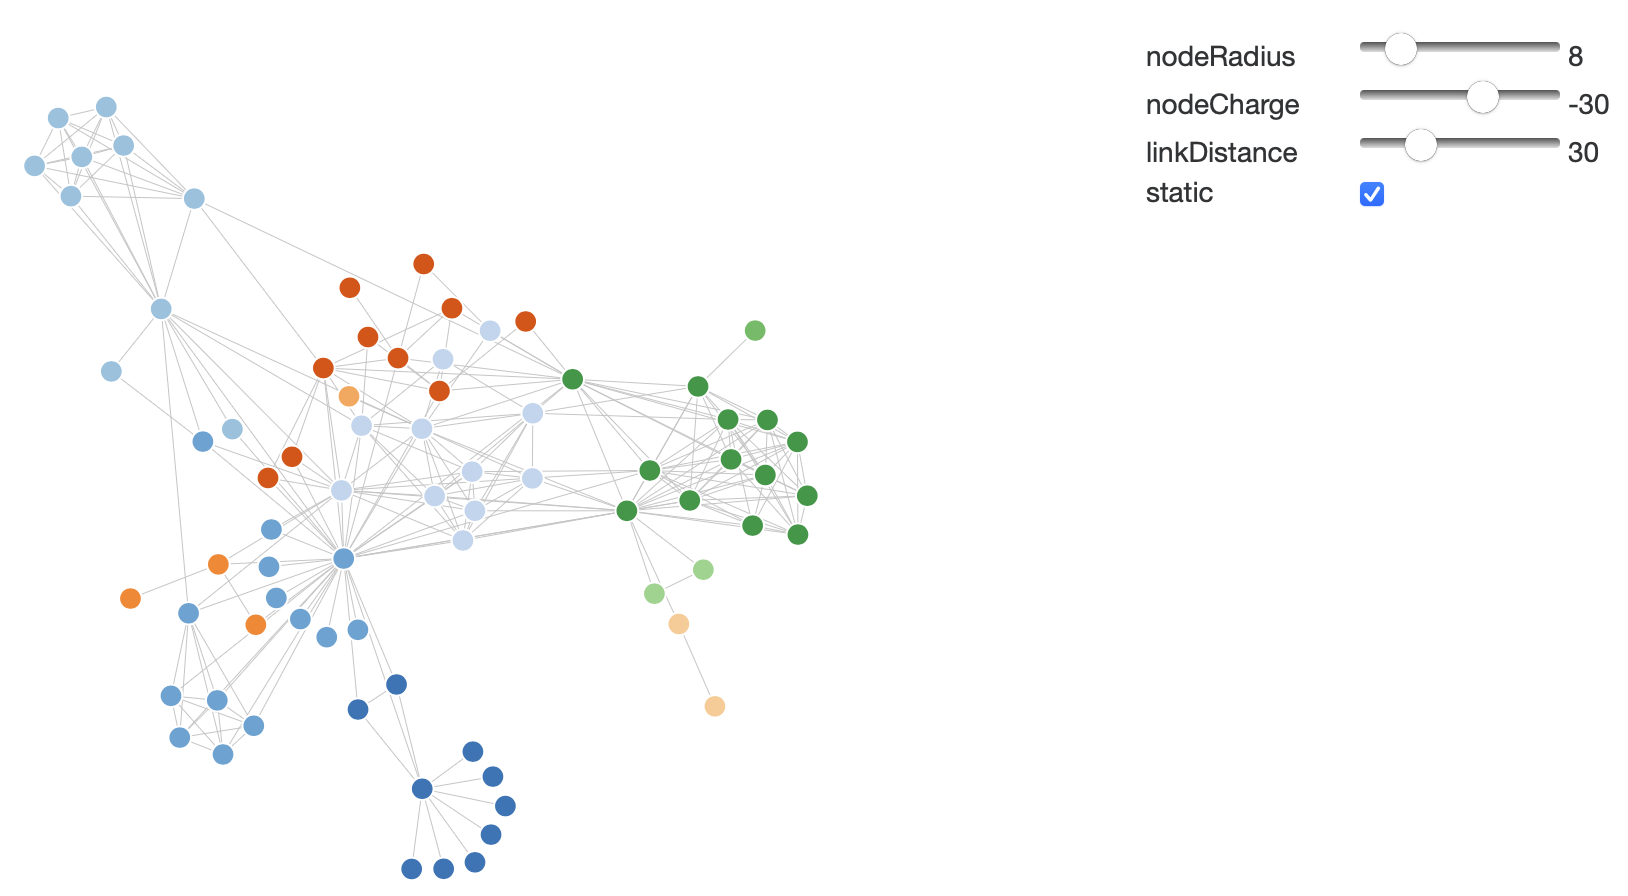
\includegraphics[width=0.8\linewidth]{./pics/vega.png}  
  \caption{Vega \cite{vega}}
  \label{fig:sub-first-vega}
\end{subfigure}
\begin{subfigure}{.45\textwidth}
  \centering
  \captionsetup{justification=centering}
  % include second image
  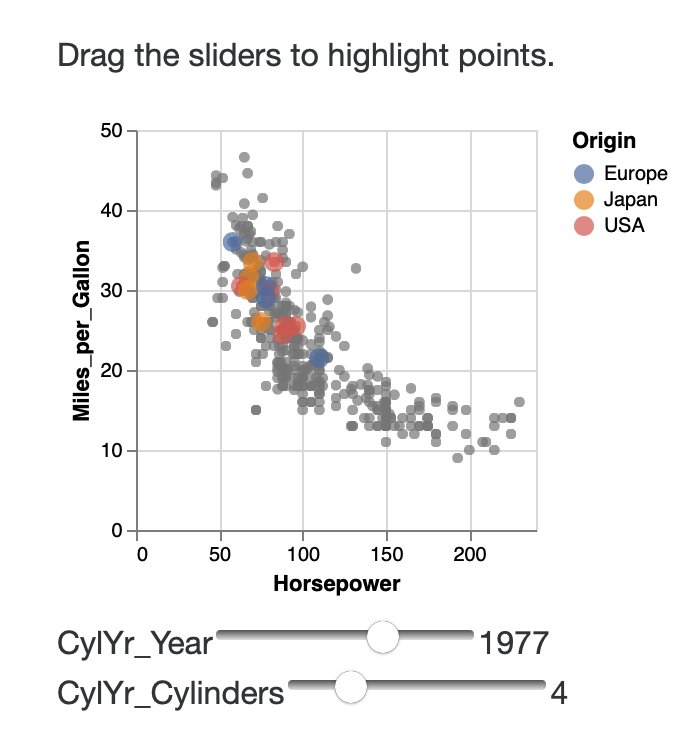
\includegraphics[width=.8\linewidth]{./pics/vegalite.png}  
  \caption{Vega-Lite \cite{vegalite}}
  \label{fig:sub-second-vegalite}
\end{subfigure}
\captionsetup{justification=centering}
\caption{Vega \& Vega-Lite Visualizations}
\label{fig:viga-vigalite}
\end{figure}

\subsection{Google Chart}
Google Chart has a rich gallery and it works across all browsers.
The most common way to use Google Chart is with simple JavaScript code that can be embedded into the web page. Users can load Google chart libraries, list all the data to be visualized, and select options to customize the charts. It is an easy-to-use library but mostly used for simple visualizations.

\begin{figure}[H]
\centering
\captionsetup{justification=centering}
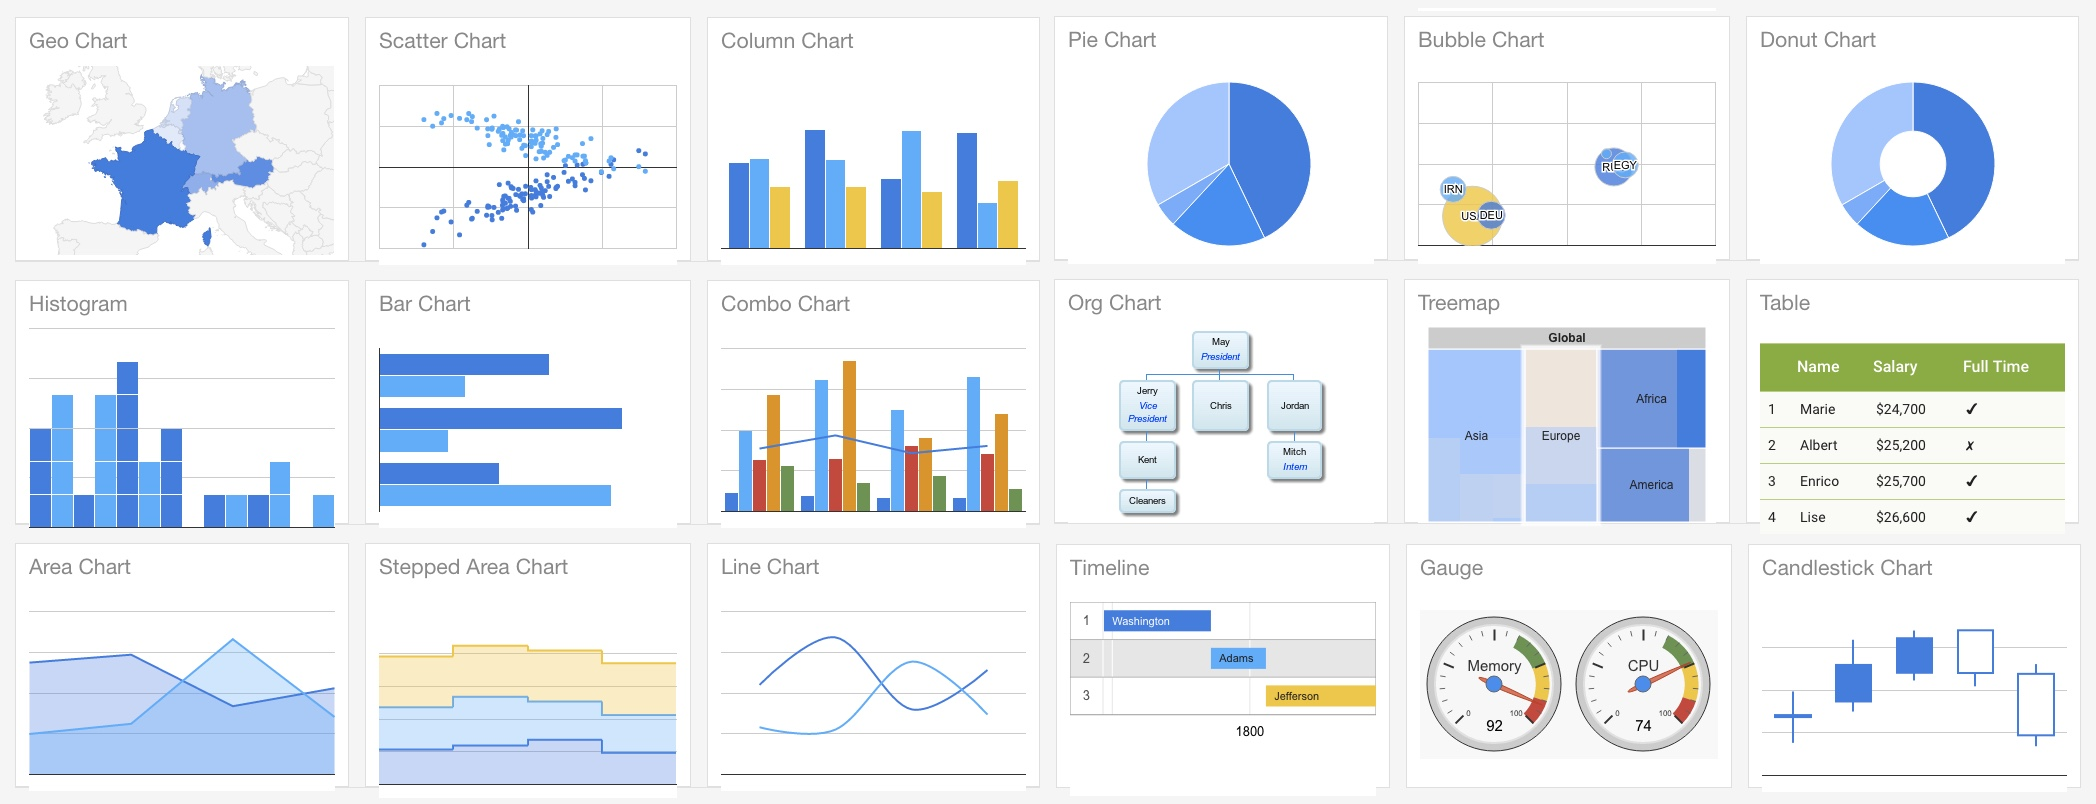
\includegraphics[width=0.7\textwidth]{./pics/charts.png}
\caption{Google Chart Gallery \cite{googlechart}}
\label{fig:google-chart}
\end{figure}

\newpage

\subsection{Datawrapper}
Datawrapper is a user-friendly, open-source web tool that can be used to create basic interactive charts. By loading the dataset into Datawrapper, it can be embedded onto a website. It is mostly used to generate pie charts, line charts, bar charts (horizontal and vertical), and maps. 

\begin{figure}[H]
\centering
\captionsetup{justification=centering}
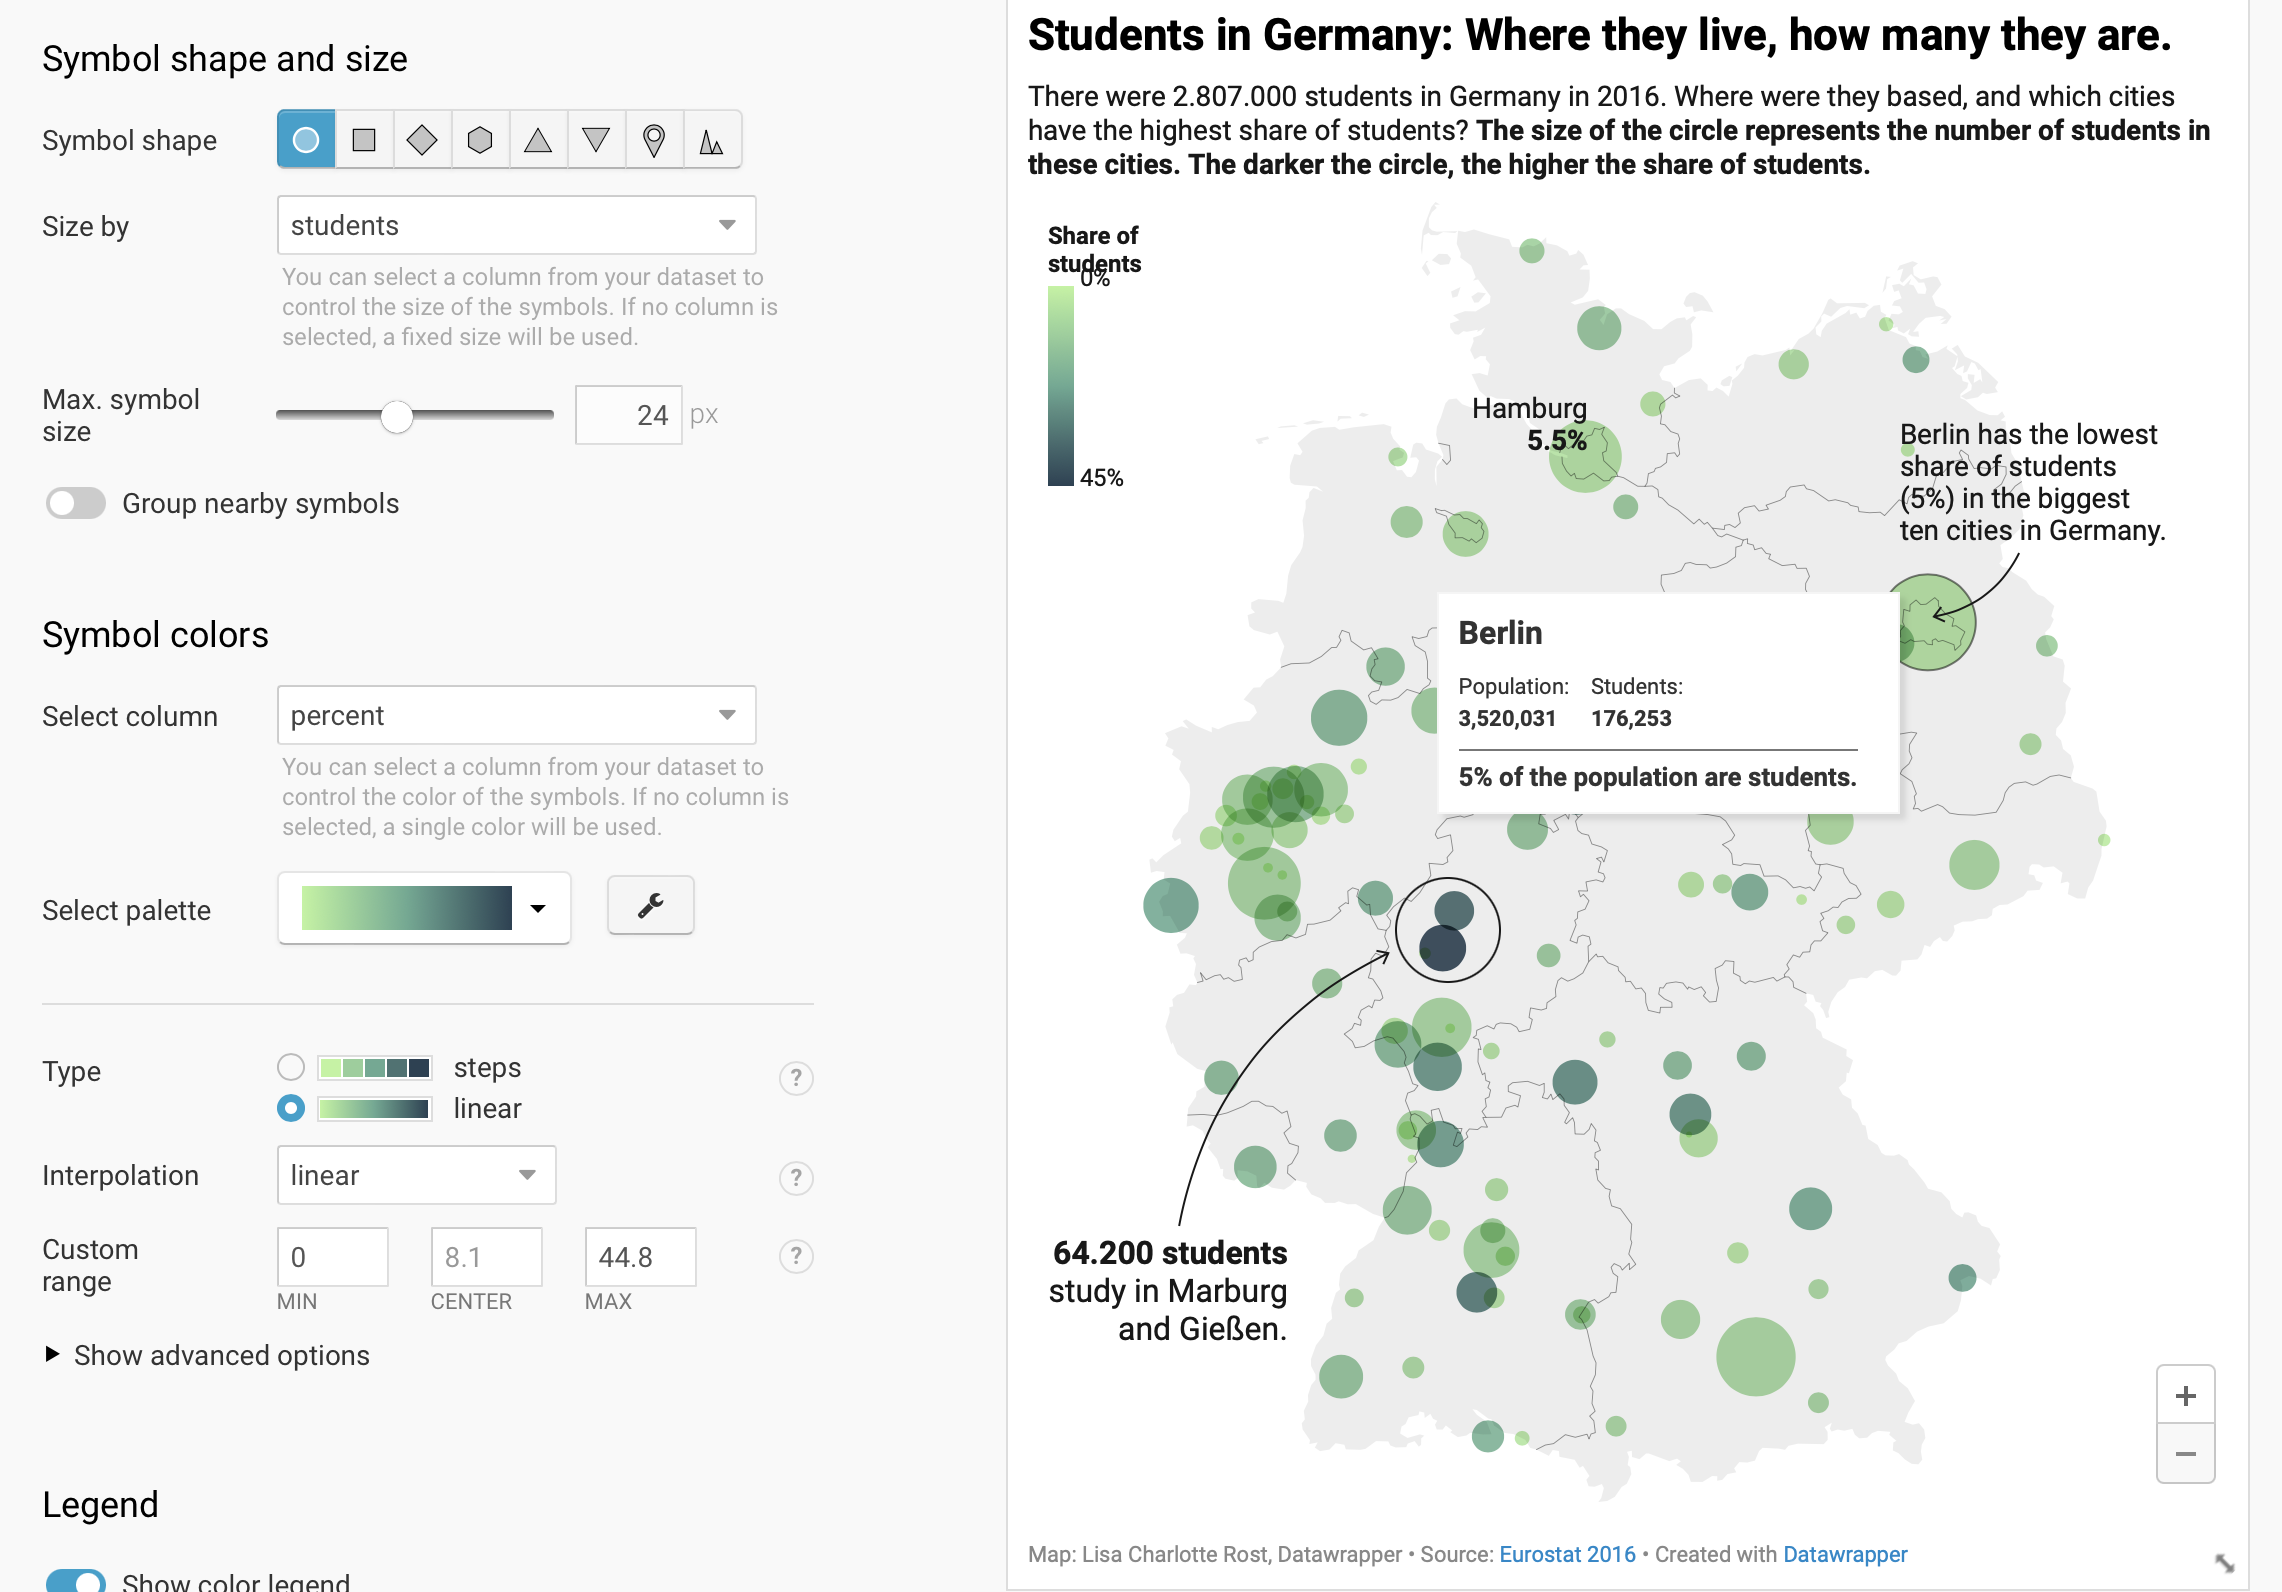
\includegraphics[width=0.7\textwidth]{./pics/datar.png}
\caption{Datawrapper interface \cite{datawrapper}}
\label{fig:datawrapper}
\end{figure}

\subsection{Canvas}
Canvas.js is a JavaScript library that can offer 30 different types of interactive charts. It is fast and can run on various devices.

\begin{figure}[H]
\centering
\captionsetup{justification=centering}
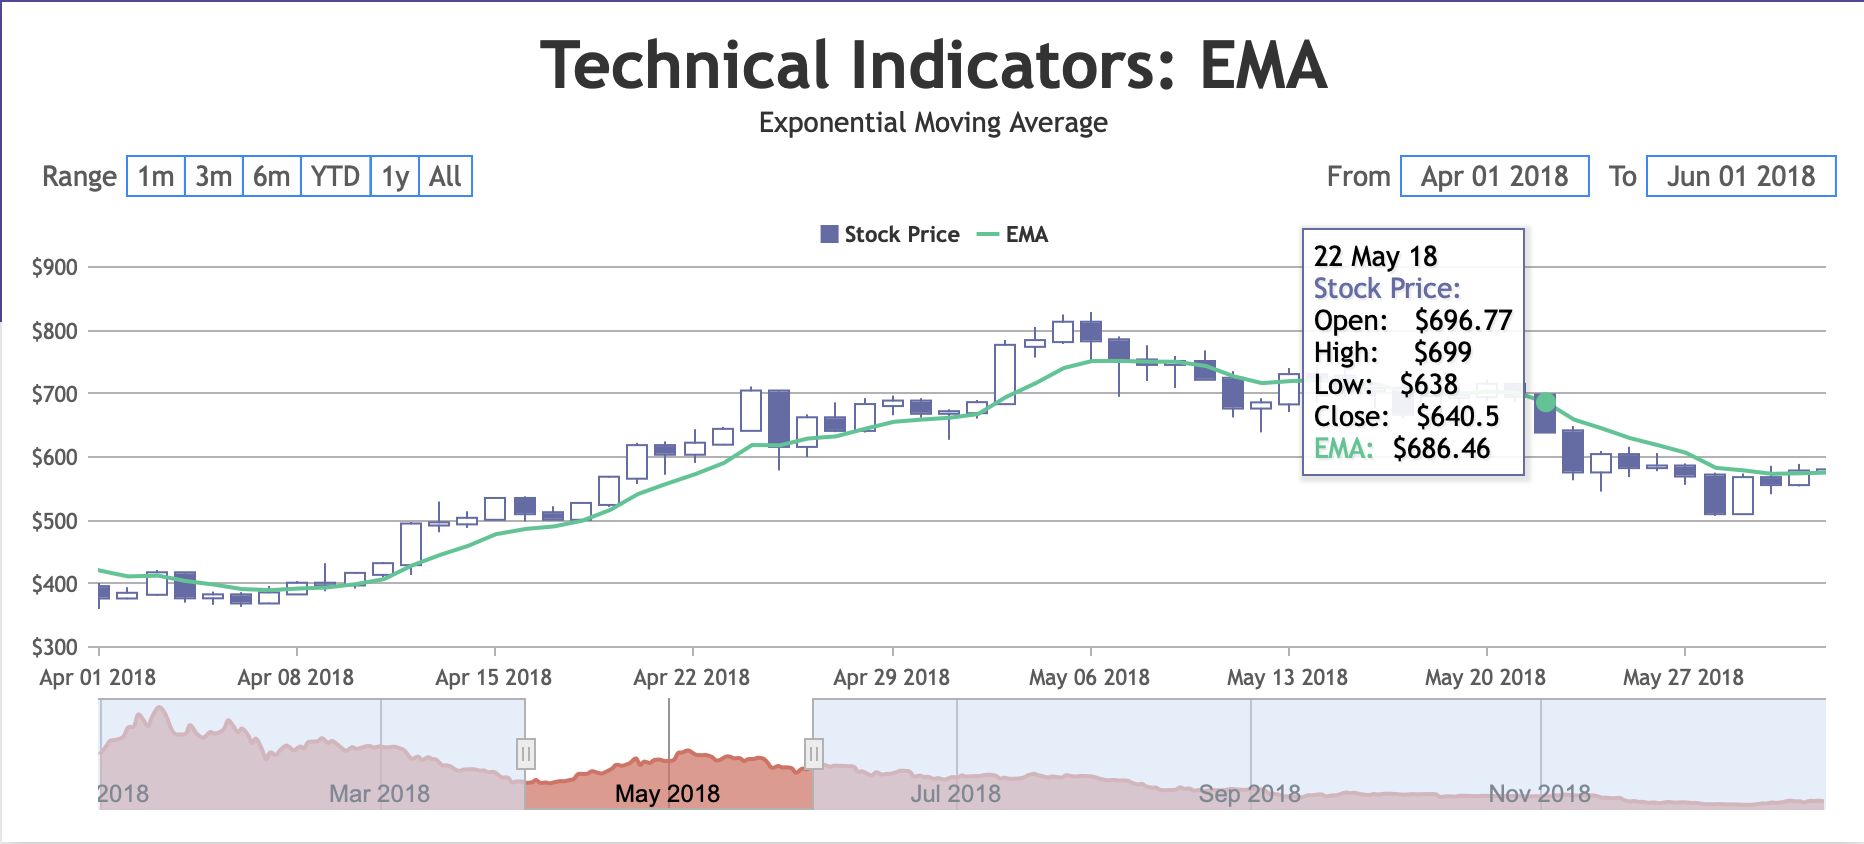
\includegraphics[width=0.7\textwidth]{./pics/canvas.png}
\caption{Canvas.js \cite{canvas}}
\label{fig:canvas}
\end{figure}



\subsection{Other Tools}

A few other tools are summarized below:

\begin{itemize}
    \item \textbf{Qlikview: }Qlik is one of the major players in the data analytics space with their Qlikview tool which is also one of the biggest competitors of Tableau \cite{qlik}.
    \item \textbf{Microsoft Power BI: }It is another leading data visualization tool like Tableau and Qlikview. It is used for data analysis and business intelligence. It is a drag and drops tool that is easy to use and it allows the user to connect to multiple data sources \cite{bi}.
    \item \textbf{Infogram: }It is a web-based data tool that requires no coding skills. Users include newsrooms, marketing teams, governments, and students \cite{infogram}.
    \item \textbf{Plotly: }It is an open-source tool that provides a list of charts with interactive nature \cite{plotly}.
    \item \textbf{Sigmajs: }It is a modern JavaScript library specialized in rendering and interacting with network graphs. It is easy to use and can draw larger graphs faster than D3 but with fewer customization \cite{sigma}.
   
\end{itemize}





